% Created 2024-12-19 Thu 18:09
% Intended LaTeX compiler: pdflatex
\documentclass[11pt]{article}
\usepackage[utf8]{inputenc}
\usepackage[T1]{fontenc}
\usepackage{graphicx}
\usepackage{longtable}
\usepackage{wrapfig}
\usepackage{rotating}
\usepackage[normalem]{ulem}
\usepackage{amsmath}
\usepackage{amssymb}
\usepackage{capt-of}
\usepackage{hyperref}
\author{Randy Ridenour}
\date{\textit{<2018-02-10 Sat>}}
\title{Truth Tables in \LaTeX{}}
\hypersetup{
 pdfauthor={Randy Ridenour},
 pdftitle={Truth Tables in \LaTeX{}},
 pdfkeywords={},
 pdfsubject={},
 pdfcreator={Emacs 29.4 (Org mode 9.8-pre)}, 
 pdflang={English}}
\usepackage{biblatex}
\addbibresource{~/Dropbox/bibtex/rlr.bib}
\begin{document}

\maketitle
Typesetting truth tables has never been easy. \LaTeX{} is the gold standard for displaying logic and mathematics, but tables are awkward to edit at best. Tables are much simpler in Microsoft Word, but displaying formulas is a horrible experience.\footnote{Apple's Pages now allows users to \href{https://support.apple.com/en-us/HT207569}{add formulas} with \LaTeX{}. It's looking like a good solution for those who like more traditional word processors.}
Here is my current workflow.

The text that I'm using this semester is \href{https://global.oup.com/ushe/product/introduction-to-formal-logic-with-philosophical-applications-9780199386482?cc=us\&lang=en\&}{Introduction to Formal Logic with Philosophical Applications} by Russell Marcus. Instead of arrows and the ampersand, it uses the horseshoe, triple bar, and dot. So, I add the following lines to my \LaTeX{} preamble to simplify entering the symbols.\footnote{The AMS \LaTeX{} packages already include a command called ``\(\lor\)'' for entering the vee or wedge.}


\begin{verbatim}
\newcommand{\lneg}{\mathord{\sim}}
\renewcommand{\land}{\bullet}
\newcommand{\lif}{\supset}
\newcommand{\liff}{\equiv}
\end{verbatim}


Then, I enter the truth table in either Excel or Numbers. For example, this would be a simple one line table determining the truth value of a formula for a given valuation:

\begin{center}
\begin{center}
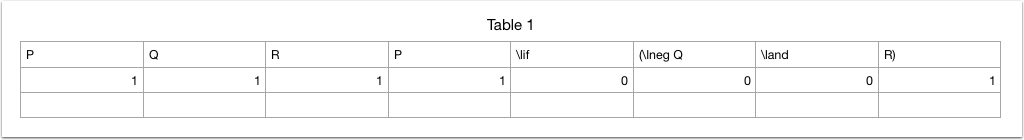
\includegraphics[width=.9\linewidth]{../images/posts/20180210-numbers-truth-table1.png}
\end{center}
\end{center}

Copy the cells that you want included in the truth table. Go to \href{http://www.tablesgenerator.com}{Tables Generator} and select ``\LaTeX{} Tables'' from the top menu bar. Below the top menu bar is a drop-down menu bar. Click on ``File'' then ``Paste table data\ldots{}'' and paste the table data. Table Generator will generate a nicely formatted \LaTeX{} table; be sure to uncheck ``Escape special \TeX{} symbols'' and select the option to remove all borders.

\begin{verbatim}
\begin{table}[]
\begin{tabular}{cccccccc}
\hline
P & Q & R & P & \lif & (\lneg Q & \land & R) \\
1 & 1 & 1 & 1 & 0    & 0        & 0     & 1  \\
\end{tabular}
\end{table}
\end{verbatim}

I delete the first and last line, leaving just the table data and the lines declaring the tabular environment: 

\begin{verbatim}
\begin{tabular}{cccccccc}
\hline
P & Q & R & P & \lif & (\lneg Q & \land & R) \\
1 & 1 & 1 & 1 & 0    & 0        & 0     & 1  \\
\end{tabular}
\end{verbatim}


At this point, typesetting will fail because the symbols need to be in math mode. So, I've found two options. The first is to put all the commands for the symbols in math mode: 

\begin{verbatim}
\begin{tabular}{cccccccc}
\hline
P & Q & R & P & \(\lif\) & (\(\lneg\) Q & \(\land\) & R) \\
1 & 1 & 1 & 1 & 0    & 0        & 0     & 1  \\
\end{tabular}
\end{verbatim}

The second option is to change ``tabular'' to ``array'' and put the entire table into math mode:

\begin{verbatim}
\[
  \begin{array}{cccccccc}
    \hline
    P & Q & R & P & \lif & (\lneg Q & \land & R) \\
    1 & 1 & 1 & 1 & 0    & 0        & 0     & 1  \\
    \end{array}
  \]
\end{verbatim}



Arrays are centered on the page. If you would prefer them printed at the left margin, add ``fleqn'' to the document class options: \texttt{\textbackslash{}documentclass[fleqn]\{article\}}. Since the array is in math mode, the letters will be italicized. I use the newtxmath font package, and it has a ``frenchmath'' option that sets the math font to non-italic. Other math fonts may have a similar option. Finally, whichever option is used, we need to add two lines. Adding a vertical line character to the table or array formatting options will place a vertical line between the valuation section and the rest of the truth table. Adding the booktabs package to the preamble will allow us to separate the sentence letters from the rest of the truth table with a ``|'' and, if desired, add a border line under the first row of the table.. This gives us the final version, 

\begin{verbatim}
\[
  \begin{array}{cc|cccccc}
    \hline
    P & Q & R & P & \lif & (\lneg Q & \land & R) \\ \midrule
    1 & 1 & 1 & 1 & 0    & 0        & 0     & 1  \\ 
    \end{array}
  \]
\end{verbatim}

which produces this: 

\begin{center}
\begin{center}

\includegraphics[width=.9\linewidth]{../images/posts/20180210-truth-table.png}
\end{center}
\end{center}
\end{document}
